\subsection{Habitat}\label{subsec:habitat}

In 1986, \textit{Habitat} was released for the Quantum Link online service for the Commodore 64 home computer. Quantum Link would later evolve into America Online~\cite{nollinger}, the first service to bring online access to the mass market.

The Commodore 64 is the most sold single computer model of all time~\cite{guinnessc64}, capturing between 30 to 40$\%$ of the United States market share at its peak~\cite{marketshare}. It was because of this popularity that the Commodore 64 was chosen as the platform for the Habitat frontend.\ \textit{Habitat}, like all Commodore 64 software, could also be played on the succeeding Commodore 128 in its backwards-compatibility mode.

\textit{Habitat} is a ``multi-player online virtual environment''~\cite{morningstar} and one of the first large-scale networked video games, supporting thousands of players in one shared world, a significant advancement from the earlier games we discussed. Players control virtual avatars which can interact with both the world around them and other players' avatars. The game provided no concrete objectives or rules but instead served as a medium for communication and interaction, allowing players to live out a virtual life. It is distinct from the bulletin board systems (BBSes) which were common at the time -- even on Quantum Link -- thanks to its virtual world, graphical representation thereof, and virtual avatars which could be separated from the human at the keyboard. Although BBSes supported messaging and online games~\cite{pcmagbbs}, there is no evidence that these had any relation to each other unlike \textit{Habitat} where virtual currency could be earned through gameplay and used to purchase cosmetic items which were visible to other players if displayed on the avatar.

\textit{Habitat} was made up of many interconnected ``regions'' which made up one screen's worth of content, containing objects and players. Players could only interact with the world and other players that were in the same region as them. Regions connected to each other with doors and teleporters, and objects could be anything from mailboxes and storekeepers to weapons and the so-called Oracle, which represented a Lucasfilm administrator who could grant special privileges or information to players. Players mainly interacted through text chat, appearing as chat bubbles over the sending avatar for all other players in the region to see.

Likely due to its much larger player capacity and the desire for data integrity, \textit{Habitat} used a client-server architecture, with users' Commodore 64 PCs operating as the client and the Quantum Link backend as the server. The backend held the representation of the world and was responsible for communicating this with the clients, handling client messages, updating world state, dealing with connections, and storing persistent data. The system operated on a zero-trust model where the server would not assume that any client data is valid, and so every message must be checked and validated before updating the world state. As such, clients would simply make requests to the server which would respond appropriately with the changes to the world state, and the client would render this. This meant that the client was only responsible for rendering, local memory management, I/O, and network communication. In comparison to the previous games, this marks the start of a trend towards offloading most of the logic to the server, freeing the client to dedicate more resources to rendering.

The lead developers strongly believed that an object-oriented paradigm was essential for multi-user worlds~\cite{morningstar} and so the entire \textit{Habitat} world was made up of objects. Objects could respond to incoming messages and change state accordingly, and were also able to initiate communication to the client on their own if they changed. If no players were in a region, objects would be written to a persistent database and unloaded from the server's memory. When a player joined a region, the server would load the relevant objects and send them to their client.

Communication was facilitated over a dial-up connection via a modem attached to the Commodore 64's RS-232 port.\ \textit{Habitat} required at least a 300 baud connection. Traffic was routed through a packet-switching network within the Quantum Link servers, which were fault-resistant Stratus minicomputers. According to information sent by Quantum Link to Lucasfilm, the expected error rate on packets was 1 per week requiring retransmission and 1 per year escaping detection~\cite{habitatsrc}. This routing could introduce between 100 and 5000ms of latency. The inter-server communication is not documented, and is outside of the scope of this review, so we will treat the backend network as a single server which corresponds with how the client and server code is written.

The source code for \textit{Habitat} is published under the MIT license by The Museum of Art and Digital Entertainment~\cite{habitatmade}. Analysis of multiple versions of the source code, documentation by the developers, notes, thoughts, and email records was done on this repository, which will make up the remainder of this section.

The Commodore 64 source code is written in the Macross 6502 cross assembler, developed by Chip Morningstar (lead developer for \textit{Habitat}) for \textit{Habitat}~\cite{macrosssrc}. The Stratus source code is written in IBM's PL/1.

Quantum Link provided software for the client to use to interface with the network, but this used one of the four 16KB memory banks of the Commodore 64, reducing the memory available for the client to store local information about the world. This limitation meant that the client software needed to be written from scratch in an interrupt-driven fashion, which is what was used in the final product. Quantum Link did not use a standardized networking protocol like TCP/IP, and had its own unique link layer packet structure.

\begin{figure}[h]
  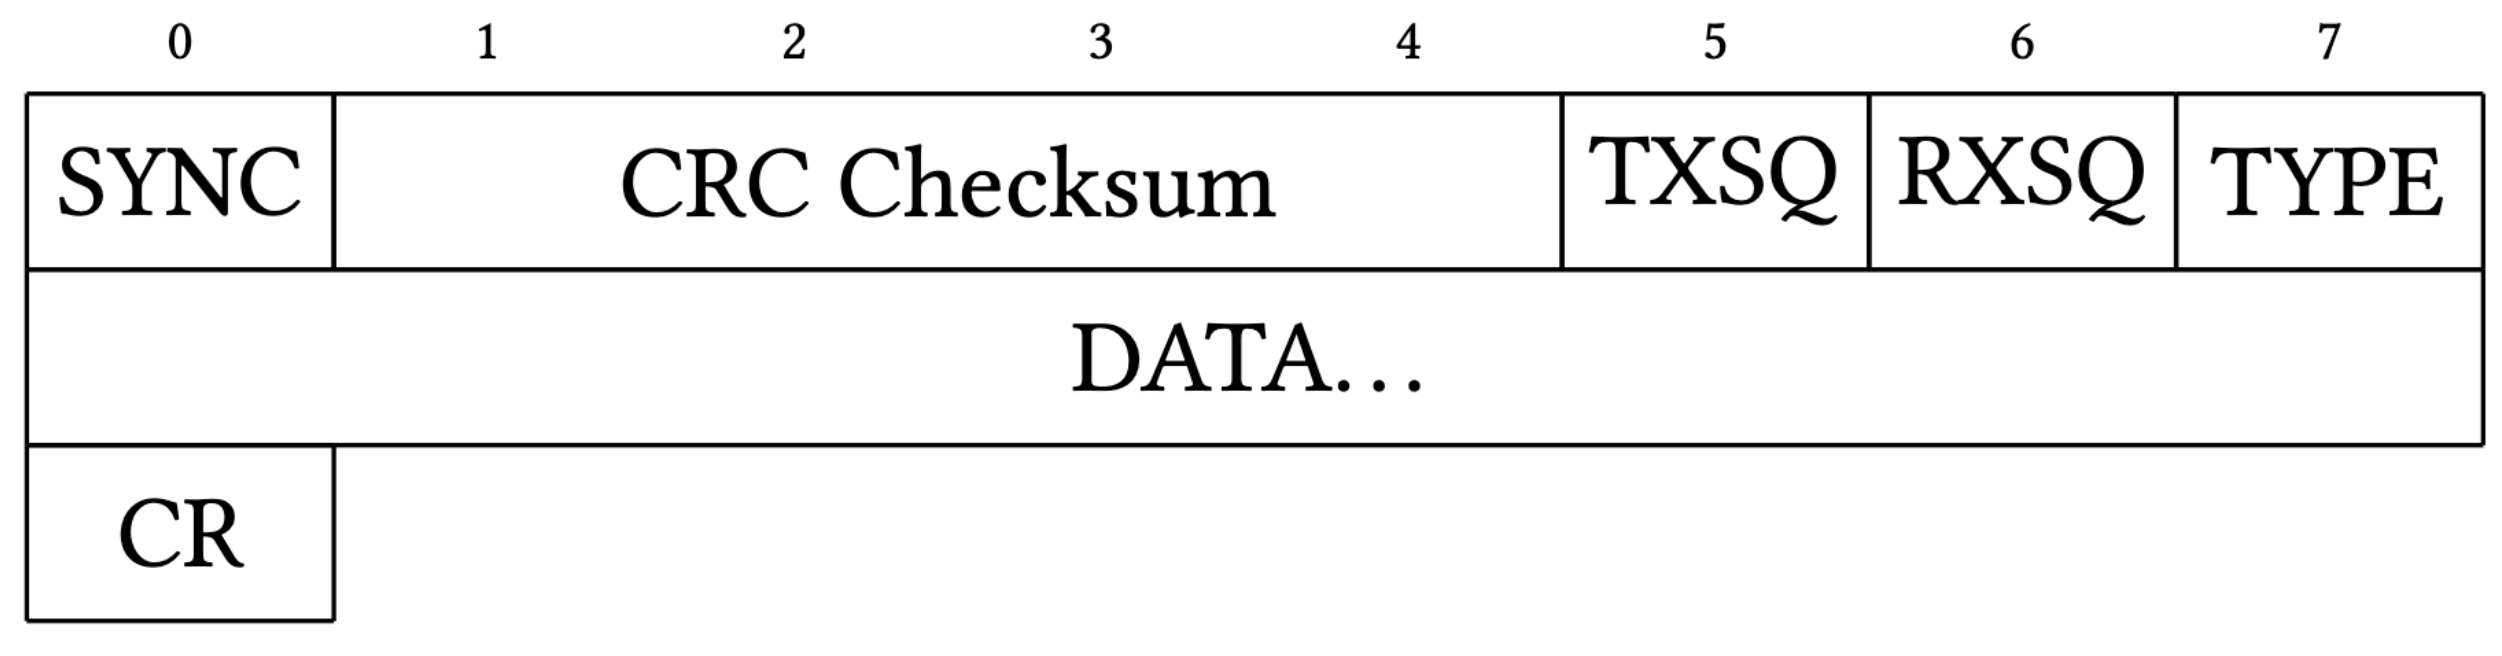
\includegraphics[scale=0.18]{figures/QLink-Diagram}
  \caption{Quantum Link link layer packet structure. Units in bytes~\cite{habitatsrc}.}
  \Description[Packet Diagram]{1 SYNC byte. 4 CRC checksum bytes. 1 TXSQ byte. 1 RXSQ byte. 1 TYPE byte. Variable DATA bytes. 1 CR.}
\end{figure}

\begin{figure}[h]
  \begin{tabular}{l l}
    SYNC& delimits start of packet\\
    CRC& 4 byte CRC checksum\\
    TXSQ& transmission sequence number\\
    RXSQ& reception sequence number\\
    TYPE& type of data\\
    DATA& payload\\
    CR& delimits end of packet
  \end{tabular}
  \caption{Description of Quantum Link link layer packet fields~\cite{habitatsrc}.}
\end{figure}

It appears the Quantum Link developers were concerned about data integrity, dedicating 2 bytes to start and end delimiters, 4 bytes to checksum, and 2 bytes to sequence numbers. This meant that it could detect corruption (using the checksum) or out-of-order transmission or reception (using sequence numbers). In total, a Quantum Link packet has 10 bytes of overhead for packet headers. This high overhead was criticized by Farmer, who suggested improvements to reduce this overhead by removing the SYNC byte and compressing the checksum, although these were not implemented.

DATA packets are considerably more complicated than those we have seen in the previous games. As such we will explore a few scenarios of packet transfer instead of describing all the details. At a high level, packets are directed from the client to a specific object on the server, which may send a message in response. The server may also send packets to the client to inform it of changes to the world state that were not triggered by the client, typically from another player's interaction with the world which is relevant to the client (\eg{} messages).

% Joining region
\begin{figure}[ht]
  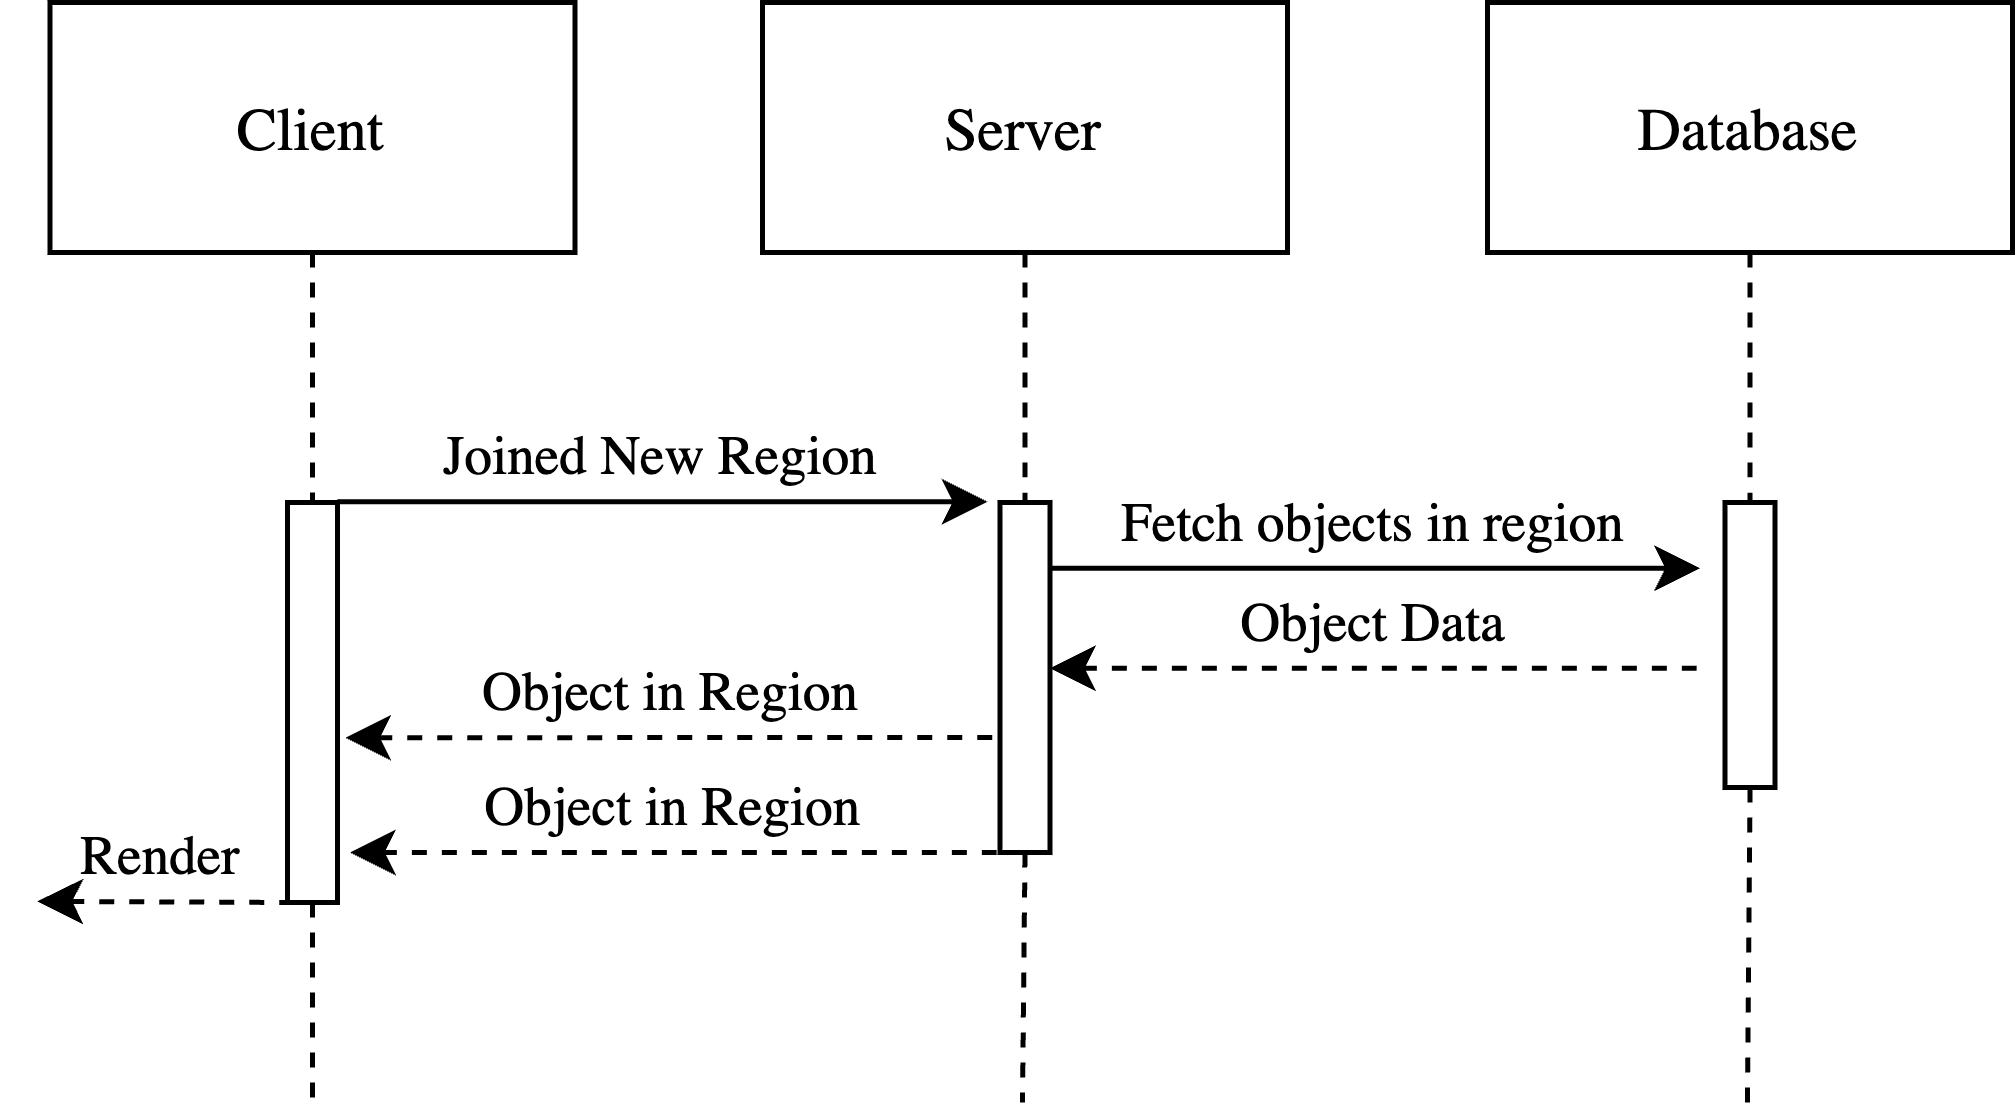
\includegraphics[width=\columnwidth]{figures/join_region}
  \caption{Joining a region with 2 objects and no other players~\cite{habitatsrc}.}
  \Description[]{}
\end{figure}

% Interacting with object
\begin{figure}[h]
  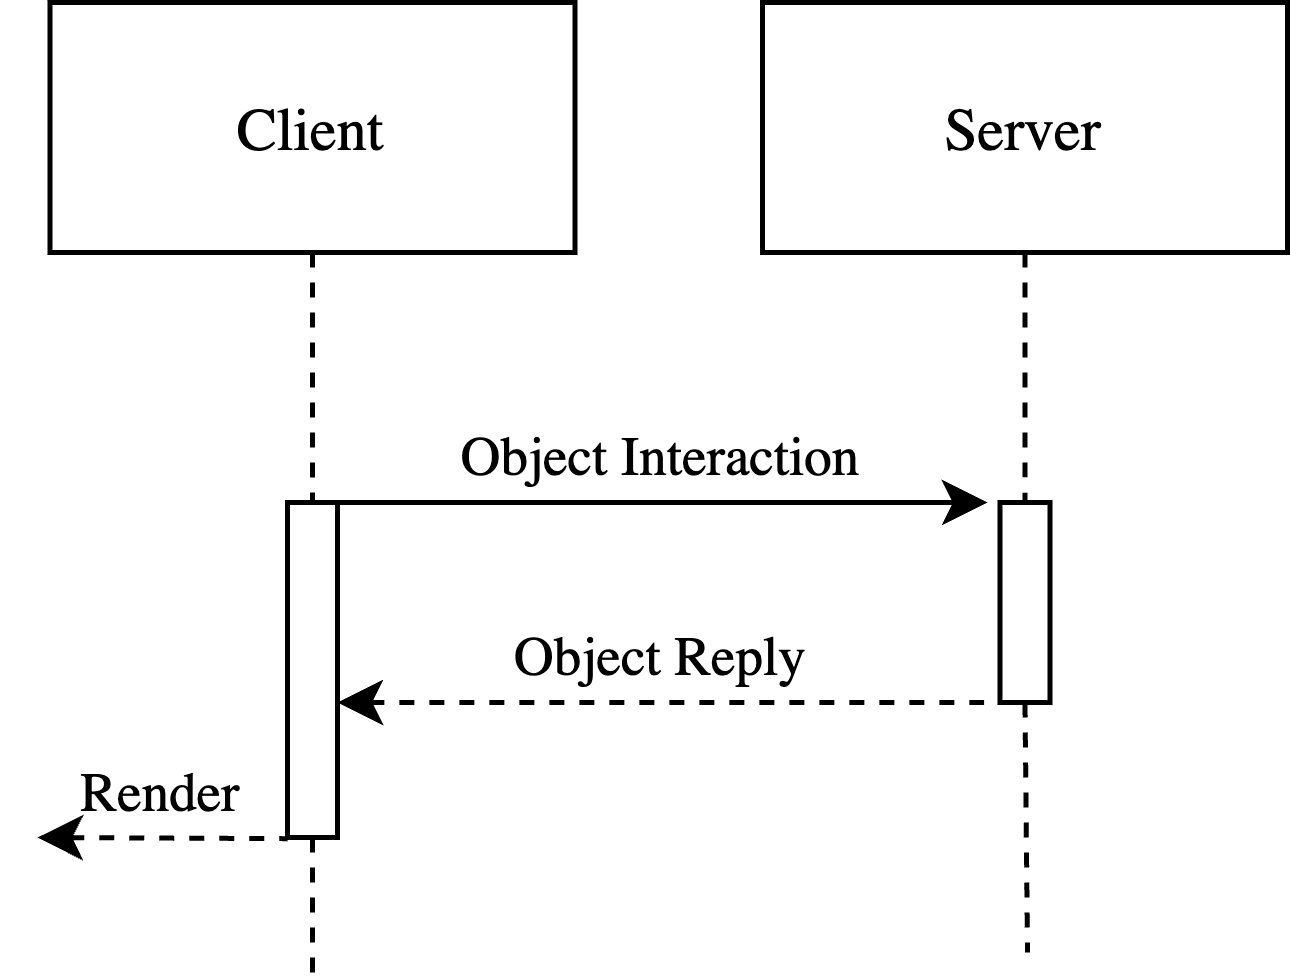
\includegraphics[width=0.66\columnwidth]{figures/interact}
  \caption{Interacting with an object~\cite{habitatsrc}.}
  \Description[]{}
\end{figure}

% Another players interaction
\begin{figure}[h]
  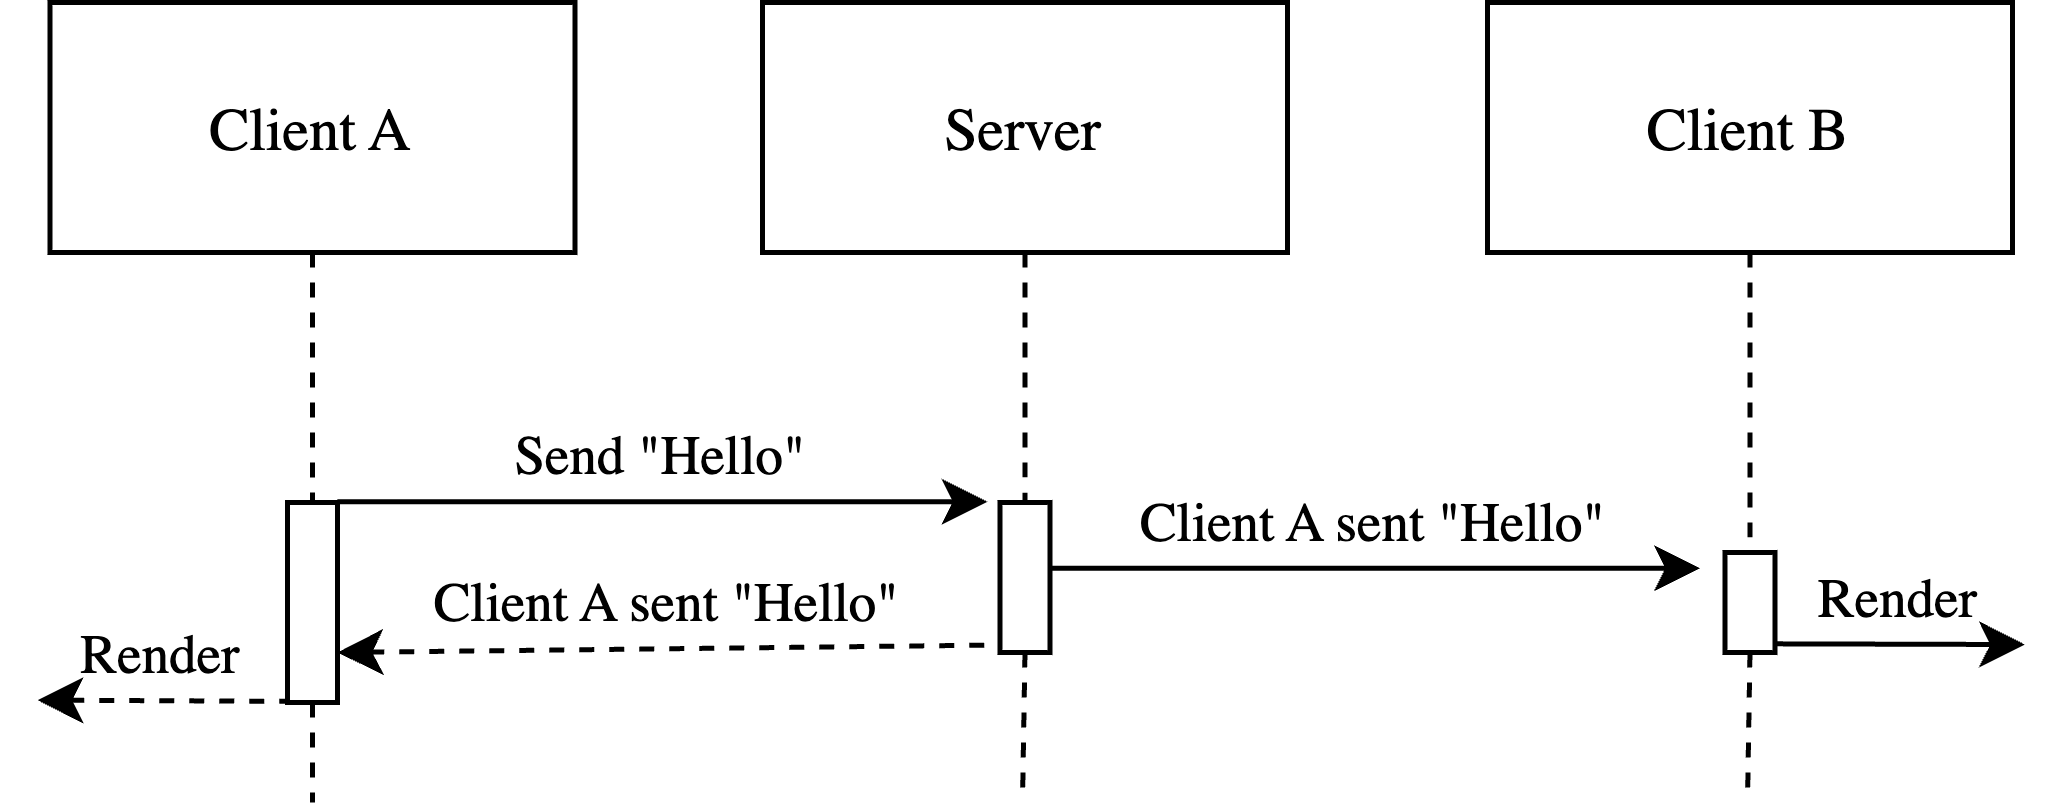
\includegraphics[width=\columnwidth]{figures/msg}
  \caption{Sending a message to a region which is received by another player~\cite{habitatsrc}.}
  \Description[]{}
\end{figure}

\textit{Habitat} featured the ability to update client-stored object data ``over-the-air'' if objects were changed or created on the server. For instance, an object sprite or list of interactions may be modified. The \textit{Habitat} client software was stored on two floppy disks -- one for program logic which would be stored in memory, then exchanged for the data disk with object data. Upon connecting to \textit{Habitat}, the client announces its presence in a message which contains the version ID of the object disk. If the server has any objects that have newer version than the clients', it would transmit the relevant blocks (storing objects) which would be written to the floppy disk. Only the final update would update the version ID of the client's block, such that if the transmission failed, the client would not assume it had all the information early, acting as a kind of transaction.

Quantum Link achieved effective communication with error correction and out-of-order protection, and \textit{Habitat} was able to utilize it to provide a novel experience to its users. However, Quantum Link was not perfect. The CRC checksum was larger than necessary and took too long to compute ``current method is unacceptably slow (cannot be over emphasized)'' -- Randall Farmer~\cite{habitatsrc}. There were also problems with flooding the Commodore 64 input buffers since the server did not check if the client was ready for more data. This naturally lead to more issues for users with a 1200 baud connection, as more data could be sent before the Commodore 64 could process it. A bug in the Quantum Link networking meant that it would not respond to client heartbeats if NAKs were pending. According to Farmer, fixing this would allow common recoveries to be performed in 2 packets instead of 6.
